%! TeX program = lualatex
\documentclass[a4paper,11pt]{article} 
% packages
\usepackage{fontspec}
\setmainfont{EB Garamond}
% for tironian et fallback
% % \directlua{luaotfload.add_fallback
% % ("emojifallback",
% %      {"Noto Serif:mode=harf"}
% % )}
% % \setmainfont{EB Garamond}[RawFeature={fallback=emojifallback}]

\setmonofont[Scale=MatchLowercase]{Deja Vu Sans Mono}
\usepackage[a4paper,left=2cm,right=2cm,top=\dimexpr15mm+1.5\baselineskip,bottom=2cm]{geometry}
\setlength{\parindent}{0pt}

\usepackage{fancyhdr}       % Headers and footers 
\fancyhead[R]{\normalfont \leftmark}
\fancyhead[L]{}
\pagestyle{fancy}

\usepackage{microtype}      % Slightly tweak font spacing for aesthetics
\usepackage[english]{babel} % Language hyphenation and typographical rules
\usepackage[final, colorlinks = true, urlcolor = blue, linkcolor = black]{hyperref} 
\usepackage{changepage}     % adjust margins on the fly

\usepackage{minted}
\usemintedstyle{algol_nu}
\usepackage{xcolor}

\usepackage{pgfplots}
\pgfplotsset{width=\textwidth,compat=1.9}

\usepackage{caption}
\newenvironment{code}{\captionsetup{type=listing}}{}
\captionsetup[listing]{skip=0pt}
\setlength{\abovecaptionskip}{5pt}
\setlength{\belowcaptionskip}{5pt}

\usepackage[yyyymmdd]{datetime}
\renewcommand{\dateseparator}{-}

\usepackage{titlesec}

\begin{document}
\begin{titlepage}
    \begin{center}
        \hrule
        \vspace*{0.6cm}
        \huge \textbf{CT326}
        \vspace*{0.6cm}
        \hrule
        \LARGE
       \vspace{0.5cm}
        PROGRAMMING III
       \vspace{0.5cm}
       \hrule
            
       \vfill
       
\includegraphics[width=\textwidth]{images/java-logo.png}
        \vfill

        \Large
       \vspace{0.5cm}
       \hrule
       \vspace{0.5cm}
       \textbf{Andreas Ó hAoḋa}
       % \vspace{0.5cm}
       % \hrule
       % \vspace{0.5cm}
            
       \normalsize
       University of Galway

       \today

       \vspace{0.5cm}
       \hrule
    \end{center}
\end{titlepage}

\pagenumbering{roman}
\newpage
\tableofcontents
\newpage
\setcounter{page}{1}
\pagenumbering{arabic}

\section{Introduction}
\subsection{Lecturer Contact Information}
\begin{itemize}
    \item Dr. Adrian Clear (\texttt{\href{mailto://adrian.clear@universityofgalway.ie}{adrian.clear@universityofgalway.ie}}).
    \item Office IT408.
\end{itemize}

\subsection{Assessment}
Continuous assessment consisting of five assignments will constitute 30\% of the overall mark. 
The exam will constitute the remaining 70\% of the overall mark.
The exam will be a written exam on pen \& paper. 
The marking will reflect this (small mistakes, e.g. missing semicolons, will not be penalised).
Practising with past exam papers is highly recommended.

\subsection{Textbook}
The textbook for this course is \emph{Java - How to Program by Deitel \& Deitel}, which is available in the University 
Bookshop.
It is not necessary to buy this book for this module.

\section{Overloading Constructors, Abstract Methods, \& Polymorphism}
\subsection{Revision}
An \textbf{object} is something upon which your program performs different operations. 
Java uses a \textbf{class} to represent objects. 
Each class has a unique name.
To create an instance of a class variable, you must use the \verb|new| operator.
A class contains members.
These may be:
\begin{enumerate}
    \item Information (or data), often called class variables. 
    \item Functions (methods) that operate on the data.
\end{enumerate}

\subsection{Overloaded Constructors}
Methods in the same class may have the same name, so long as they have different \textbf{parameter lists}.
An overloaded constructor is creating by declaring more than one constructor for one class, each with distinct parameter lists.

\subsection{Class Inheritance}
When your programs use inheritance, you use a \textbf{superclass} to derive a new class. 
The new class inherits the superclass's members.
To initialise class members for an extended class (called a \textbf{sub-class}), the application invokes the super class and 
sub-class constructors.
The \verb|this| \& \verb|super| keywords are used to refer to the current class \& the superclass, respectively.
\\\\
There are three types of members: \textbf{public}, \textbf{private}, \& \textbf{protected}.
\begin{figure}[H]
    \centering
    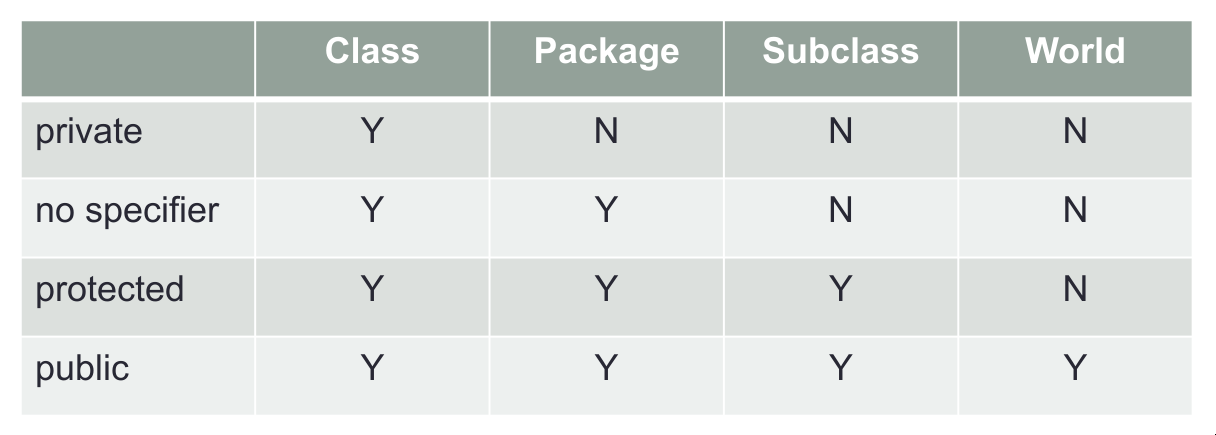
\includegraphics[width=0.8\textwidth]{./images/access_level_specifiers.png}
    \caption{Access Level Specifiers}
\end{figure}

The keyword \verb|final| is used to indicate that a class member cannot be overridden or modified.


\subsection{Abstract Classes}
An \textbf{abstract} class is one that cannot be instantiated. 
They are declared with the keyword \verb|abstract|, e.g.:

\mintinline{Java}{public abstract class Employee}.
Abstract classes can have instance data and non-abstract (concrete) methods for sub-classes.
Abstract classes can have constructors for sub-classes to initialise inherited data.
Sub-classes of an abstract class must be also be abstract, and declared with the keyword \verb|abstract|.

\section{Command-Line Programming}
\subsection{Solving Common Coding Problems}
\begin{itemize}
    \item   Problem: The compiler complains that it can't find a class
            \begin{itemize}
                \item   Make sure that you've imported the class or its package. 
                \item   Unset the \verb|CLASSPATH| environment variable, if it's set.
                \item   Make sure that you're spelling the class name exactly the same as it's declared. 
                \item   Also, some programmers use different names for the class name from the \verb|.java| filename. 
                        Make sure that you're using the class name and not the filename.
                \end{itemize}

    \item   Problem: The interpreter says that it can't find one of my classes.
            \begin{itemize}
                \item   Make sure that you specified the class name, not the class file name, to the interpreter.
                \item   Unset the \verb|CLASSPATH| environment variable, if it's set.
                \item   If your classes are in packages, make sure that they appear in the correct sub-directory.
                \item   Make sure that you're invoking the interpreter from the directory in which the \verb|.class| file is 
                        located.
            \end{itemize}

    \item   Generally, don't compare floating-point numbers using \verb|==|.
            Remember that floats are only approximations of the real thing, so therefore, the greater than \& less than 
            operators (\verb|>| \& \verb|<|) are often more appropriate when conditional logic is performed on floating-point 
            numbers.
    \item   Don't overuse the negation operator \verb|!| as it can be confusing \& error-prone.
\end{itemize}

\section{Testing}
\textbf{Testing} is the systematic process of analysing a system or system component to detect the differences between 
specified (required) behaviour \& observed (existing) behaviour. 
Testing attempts to show that the implementation of a system is inconsistent with the desired functionality. 
The goal is to design tests that exercise defects in the system and to reveal problems. 
We cannot test everything in a large system, so there are always trade-offs required with budget \& time constraints.

\subsection{Levels of Testing}
\begin{itemize}
    \item   \textbf{Unit testing} involves testing individual  classes \& mechanisms. 
    \item   \textbf{Integration testing} involves testing groups of classes or components and the interfaces between them. 
    \item   \textbf{System testing} involves integration testing the system as a whole to check it meets the requirements. 
\end{itemize}

\subsection{Test-Driven Development (TDD)}
\textbf{Test-Driven Development (TDD)} is a software development process that relies on the repetition of a very short 
development cycle. 
The general rationale behind this methodology is ``first write the test, then the code'' such that the tests \emph{drive} the 
development of your code. 
TDD tries to find faults in participating objects and/or sub-systems with respect to the use cases from the use case model.
\begin{figure}[H]
    \centering
    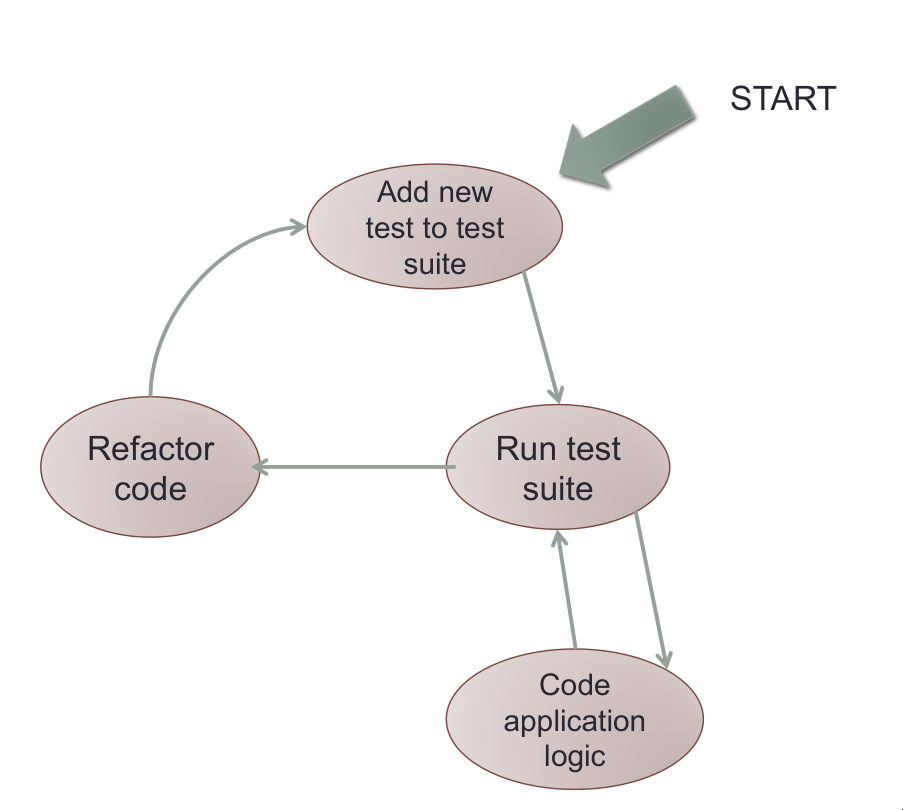
\includegraphics[width=0.6\textwidth]{./images/tdd_cycle.png}
    \caption{The TDD Cycle}
\end{figure}

Any test will initially fail; We then write the minimum amount of code to make our test pass. 
We refactor our application and test the code before moving onto the next test.
We build a test suite as our implementation progresses.

\subsubsection{Test Cases}
A \textbf{test component} is a part of the system that can be isolated for testing. 
This could be an object, a group of objects, or one or more subsystems. 
\textbf{Unit testing} finds differences between a specification of an object and its realisation as a component.
\textbf{JUnit} is a unit testing framework for test-driven development in Java, which is available in Eclipse out-of-the-box.
\\\\ 
A \textbf{test case} is a set of inputs \& expected results that exercises a test component with the purpose of causing 
failures \& detecting faults. 
\textbf{Black box tests} focus on the input/output behaviour of the component, i.e. the functionality, not the internal aspects. 
\textbf{White box tests} focus on the internal structure \& dynamics of the component.
\begin{figure}[H]
    \centering
    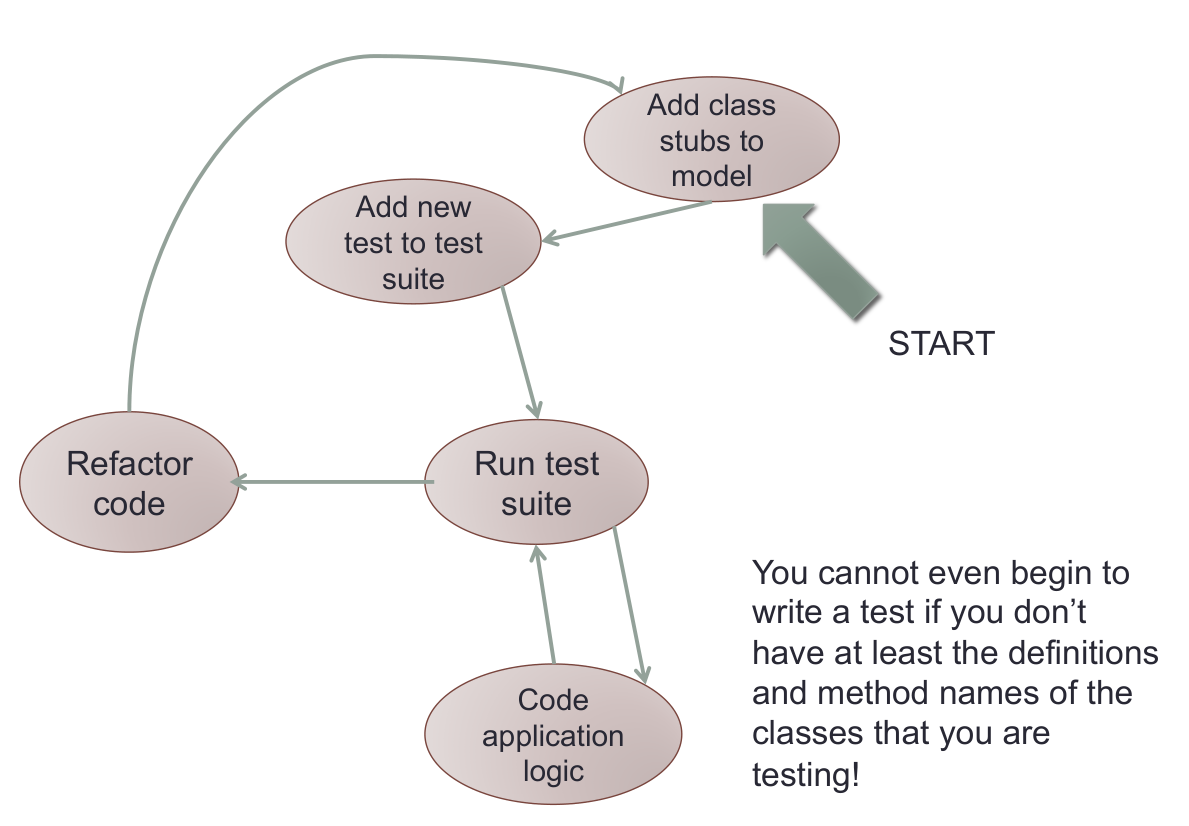
\includegraphics[width=0.6\textwidth]{./images/tdd_cycle_oo.png}
    \caption{The TDD Cycle in Object-Oriented Development}
\end{figure}

\subsubsection{Assert Methods}
\begin{code}
\begin{minted}[texcl, mathescape, linenos, breaklines, frame=single]{Java}
assertTrue(boolean test)
assertTrue(String message, boolean test)

assertFalse(boolean test)
assertFalse(String message, boolean test)

assertEquals(Object expected, Object actual)
assertEquals(String message, Object expected, Object actual)

assertSame(Object expected, Object actual)
assertSame(String message, Object expected, Object actual) 

assertNotSame(Object expected, Object actual)
assertNotSame(String message, Object expected, Object actual) 

assertNull(Object object)
assertNull(String message, Object object) 

assertNotNull(Object object)
assertNotNull(String message, Object object) 

fail()
fail(String message) 
\end{minted}
\end{code}

\section{Throwing \& Handling Exceptions}
Alternatives to exception handling include using no error handling or just exiting the application on error.

\subsection{Basics of Java Exception Handling}
Code that could generate errors are put in \verb|try| blocks, and the code for handling the error are enclosed in a 
subsequent \verb|catch| block.
The \verb|finally| block always executes with or without an error.
The \verb|throws| keyword is used to specify the exceptions which a method might throw if a problem occurs.
An exception is thrown when a method detects an error, the exception handler processes the error. 
The error is thus considered \textbf{caught} \& \textbf{handled} in this model.
Control moves from the \verb|try| blocks to the \verb|catch| block(s).

\begin{code}
\begin{minted}[texcl, mathescape, linenos, breaklines, frame=single]{Java}
try {
    // statements that may throw an exception
}
catch (ExceptionType exceptionReference) {
    // statemetns to process the exception
}
// a `try` is followed by any number of `catch` blocks 
catch (ExceptionType exceptionReference) {
    // statemetns to process the exception
}
\end{minted}
\caption{\texttt{try} Blocks}
\end{code}

\subsection{Throwing \& Catching Exceptions}
The \verb|throw| statement is used to indicate that an exception has occurred. 
The operand of the \verb|throw| statement is any class that is derived from the class \verb|Throwable|. 
The sub-classes of \verb|Throwable| are \verb|Exception| (used for problems that should be caught) \& \verb|Error| 
(used for serious problems that should not be caught).
\\\\
An exception is caught by a \textbf{handler}.
The program will terminate if there is no appropriate handler for an exception.
A single \verb|catch| statement can handle multiple exceptions. 
\\\\
The \verb|throws| clause lists the exceptions thrown by a method. 
\begin{code}
\begin{minted}[texcl, mathescape, linenos, breaklines, frame=single]{Java}
int functionName (paremeterList) throws ExceptionType1, ExceptionType2 {
    // method body
}
\end{minted}
\caption{\texttt{throws} Clause}
\end{code}

\verb|RunTimeExceptions| occur during the execution of a program, e.g. \verb|ArrayIndexOutOfBoundsException| \& \\
\verb|NullPointerException|. 

\subsection{Checked \& Unchecked Exceptions}
\textbf{Unchecked Exceptions} (or runtime exceptions) represent unrecoverable errors that occur during the execution of a 
program. 
These include sub-classes of \verb|RuntimeException| such as \verb|NullPointerException|.
(A full list of runtime exceptions can be found here: \url{https://docs.oracle.com/javase/8/docs/api/java/lang/RuntimeException.html})
It is not necessary to add the \verb|throws| declaration for this type of exceptions and it is not necessary to handle 
them.
\\\\ 
\textbf{Checked Exceptions} are caught at compile time. 
All exceptions other than sub-classes of \verb|RuntimeException| are checked exceptions. 
An example of a checked exception is \verb|FileNotFoundException|. 
Checked exceptions are predictable \& recoverable.
They must be handled in the method body, either with a \verb|try|/\verb|catch| statement or by re-throwing. 
It is necessary to add the \verb|throws| declaration for this type of exceptions

\subsection{Finalizers}
We can throw an exception if a constructor causes an error.
The \verb|finalize| method is called the first time that garbage collection is attempted on an object. 
It will be called a maximum of one times (regardless of whether or not the garbage collection was successful), but
won't necessarily ever be called.
However, since this won't necessarily be called, it's better not to use it when a resource needs to be released. 
Instead, one should use the \verb|finally| statement after a \verb|try|/\verb|catch| block. 
This always executes, and can be used to release resources.

\subsection{Exception Methods}
The \verb|printStackTrace()| method of an exception is used to print the method call stack. 
The \verb|getMessage()| method retrieves the \verb|informationString| from an exception.

\section{Unit Testing in Java}
We should test single units of functionality in isolation. 
Unit tests are not integration tests. 
There should be multiple tests for a single piece of logic, one for each scenario. 
Each test will cover a single scenario and a single piece of logic.

\subsection{Unit Testing Techniques}
\subsubsection{Equivalence Testing}
In \textbf{equivalence testing}, possible inputs are partitioned into equivalence classes and a test case is selected for 
each class. 
This minimises the number of test cases. 
Systems usually behave in similar ways for all members of a class.

\subsubsection{Boundary Testing}
\textbf{Boundary testing} is a special case of equivalence testing that focuses on the conditions at the boundary of the 
equivalence classes. 
Instead of selecting any element in the equivalence class, boundary testing requires that the elements be selected from the 
``edges'' of the equivalence class. 
The assumption is that developers often overlook special cases at the boundary of the equivalence classes. 

\subsubsection{Path Testing}
\textbf{Path testing} exercises all the possible paths through the code at least once, which should cause most faults to 
trigger failures. 
This requires knowledge of the source code \& data structures.
\\\\ 
\textbf{Code coverage} is a measure of how many lines of your code are executed by automated tests. 
It is impractical to achieve 100\% code coverage for large projects.

\subsection{Testing Code with Dependencies}
Often, the application logic that we want to test will have some dependencies on external services or components. 
In Unit Testing, we want to isolate our component under test from any dependencies (otherwise, we would be doing 
\textbf{integration testing}). 
This is problematic as our application logic won't work without its dependencies. 
The solution to this problem is to create a \textbf{stub} to simulate the functionality of this external component.

\subsection{TDD Guidelines}
\begin{itemize}
    \item   Test the expected outcomes of an example.
    \item   Think about examples \& outcomes, not code or how it should work in detail.
    \item   Don't pre-judge design -- let your tests drive it. 
    \item   Write the minimum code to get your tests to pass. 
    \item   Each test should validate one single piece of logic.
\end{itemize}

\section{Strings}
Strings allow us to store alphanumeric characters within a variable. 
In Java, you do not use the \verb|'\0'| (null) character to indicate the end of a \verb|String| object, as you would in C or 
C++. 
The \verb|String| object itself keeps track of the number of characters it contains. 
The \verb|String| \verb|length()| method is the number of characters that a \verb|String| object contains.
\begin{itemize}
    \item   \verb|int length()| returns the length of the \verb|String|. 
    \item   \verb|char charAt(int index)| returns the \verb|char| value at the specified index. 
    \item   \verb|boolean isBlank()| returns \verb|true| if the \verb|String| is empty or contains only whitespace codepoints,
            otherwise it returns \verb|false|.
    \item   \verb|boolean startsWith(String prefix)| tests if the \verb|String| starts with the specified prefix. 
    \item   \verb|boolean matches(string regex)| tells whether or not the \verb|String| matches the given regular expression.
\end{itemize}

\subsection{Creating Strings}
\begin{minted}[texcl, mathescape, linenos, breaklines, frame=single]{Java}
String myString = "Hello world!"; 
String myString = new String();
char [] ct326Array = { ‘C', ‘T', ‘3', ‘2', ‘6' }; 
String ct326String = new String(ct326Array);

String fs = tring.format("The value of the float variable is %f, while the value of the integer variable is %d, and the string is %s", floatVar, intVar, stringVar); 
\end{minted}

\subsection{Concatenating Strings}
The \verb|+| operator lets your program concatenate one String's contents onto another. 
When you concatenate a numeric value, e.g. of type \verb|int| or \verb|float|, Java automatically calls a method called 
\verb|toString()| on the numeric value to convert the value into a character String.
To simplify the output of class-member variables, you can write a \verb|toString()| method for the classes you create; 
In the same way as for built-in types, the \verb|toString| method will be called automatically for your class.
The \mintinline{Java}{String concat(String str)} method of the \verb|String| class concatenates the specified String to the
end of this String.

\subsection{Comparing Strings}
The \mintinline{Java}{int compareTo(String anotherString)} \verb|String| method compares two \verb|String|s lexicographically.

The \mintinline{Java}{boolean equalsIgnoreCase(String anotherString)} \verb|String| method compares this \verb|String| to 
another \verb|String|, ignoring letter case.

\subsection{Manipulating Strings}
\begin{itemize}
    \item   \mintinline{Java}{String substring(int beginIndex, int endIndex)} returns a \verb|String| that is a sub-String 
            of the \verb|String| on which the method was called.
    \item   \mintinline{Java}{String [] split(String regex)} splits the \verb|String| around matches of the given 
            regular expression
    \item   \mintinline{Java}{String strip()} returns this \verb|String| but with all leading \& trailing whitespace removed.
    \item   \mintinline{Java}{String replace(char oldChar, char newChar)} returns a \verb|String| resulting from replacing all
            of \verb|oldChar| in this \verb|String| with \verb|newChar|.
\end{itemize}

\subsection{String Handling}
\verb|String| objects are \textbf{immutable} -- They cannot be changed once they've been created.
The \verb|java.lang| package provides a different class, \verb|StringBuffer|, which you can use to create \& manipulate 
character data on the fly.

\section{Nested Classes}
In Java, it is possible to define a class as a member of another class. 
Such a class is called a \textbf{nested class} and is of the following form:
\begin{minted}[texcl, mathescape, linenos, breaklines, frame=single]{Java}
class EnclosingClass {
    ...
    class ANestedClass {
        ...
    }
}
\end{minted}

Nested classes are used to reflect \& to enforce the relationship between two classes. 
You should define a class within another class when the nested class makes sense only in the context of its enclosing 
class or when it relies on the enclosing class for its function. 
For example, a text cursor might only make sense in the context of a text component. 
\\\\
As a member of its enclosing class, a nested class has a special privilege: it has unlimited access to its enclosing 
class's members, even if they are declared \verb|private|. 

\subsection{Static \& Inner Classes}
Like other class members, a nested class can be declared \verb|static|:
\begin{itemize}
    \item   A static nested class is simply called a \textbf{static nested class}.
    \item   A non-static nested class is just called an \textbf{inner class}
\end{itemize}
\begin{minted}[texcl, mathescape, linenos, breaklines, frame=single]{Java}
class EnclosingClass {
    ...
    static class StaticNestedClass {
        ...
    }
    class InnerClass {
        ...
    }
}
\end{minted}

As with static methods \& variables (which we call class methods \& variables), a static nested class is associated with 
its enclosing class. 
Like class methods, a static nested class cannot refer directly to instance variables or methods defined in its 
enclosing class; It can only use them through an object reference.
As with instance methods \& variables, an inner class is associated with an instance of its enclosing class and has
direct access to that object's instance variables \& methods.
\\\\
The interesting feature of the relationship between the inner class \& the enclosing class is \emph{not} that the inner
class is syntactically defined within the enclosing class. 
Rather, it's that an instance of the inner class can only exist within an instance of the enclosing class, and that it 
has direct access to the instance variables \& methods of its enclosing instance. 
You may encounter nested classes of both static \& inner types in the Java platform API and be required to use them. 
However, most nested classes that you write will probably be \textbf{inner classes}.

\subsection{Using Anonymous Inner Classes}
Using a Tokenizer, partition a \verb|String| into individual sub-strings using a \textbf{delimiter}. 
To do this, Java offers \\ \verb|java.util.StringTokenizer|

\begin{code}
\begin{minted}[texcl, mathescape, linenos, breaklines, frame=single]{Java}
// Fig. 10.20: TokenTest.java
// Testing the StringTokenizer class of the java.util package

// Java core packages
import java.util.*;
import java.awt.*;
import java.awt.event.*;

// Java extension packages
import javax.swing.*;

public class TokenTest extends JFrame {
    private JLabel promptLabel;
    private JTextField inputField;
    private JTextArea outputArea;

    // set up GUI and event handling
    public TokenTest()
    {
        super( "Testing Class StringTokenizer" );

        Container container = getContentPane();
        container.setLayout( new FlowLayout() );

        promptLabel = new JLabel( "Enter a sentence and press Enter" );
        container.add( promptLabel );

        inputField = new JTextField( 20 ); // inputField contains String to be parsed by StringTokenizer

        inputField.addActionListener(
            // anonymous inner class
            new ActionListener() {
                // handle text field event 
                public coid actionPerformed(ActionEvent event) 
                {
                    String stringToTokenize = event.getActionCommand();
                    StringTokenizer tokens = new StringTokenizer( stringToTokenize ); // Use StringTokenizer to parse String stringToTokenize with default delimiters "{\textbackslash}n{\textbackslash}t{\textbackslash}r"

                    outputArea.setText( "Number of elements: " + tokens.countTokens() + "\nThe tokens are:\n" ); // count number of tokens

                    // apend next token to outputArea as long as tokens exist
                    while ( tokens.hasMoreTokens() )
                        outputArea.append( tokens.nextToken() + "\n" );
                } 
            }   // end anonymous inner class
        );  // end call to addActionListener

        container.add( inputField ); 

        outputArea = new JTextArea( 10, 20 );
        outputArea.setEditable( false );
        container.add( new JScrollPane( outputArea ) );

        setSize( 275, 260 );  // set the window size
        show();               // show the window
    }

    // execute application
    public static void main( String args[] )
    {
        TokenTest application = new TokenTest();
        application.addWindowListener(
            // anonymous inner class
            new WindowAdapter() {
                // handle event when user closes window
                public void windowClosing( WindowEvent windowEvent )
                {
                    System.exit( 0 );
                }
            }  // end anonymous inner class
        ); // end call to addWindowListener
    }  // end method main
}  // end class TokenTest
\end{minted}
\caption{\texttt{TokenTest.java}}
\end{code}

\section{Enums}
An \textbf{enumerated type} is a type whose legal values consist of a fixed set of constraints. 
Common examples include the cardinal directions, the days of the week, etc.
In Java, you define an enumerated type by using the \verb|enum| keyword. 
For example, you would specify a days-of-the-week enumerated type as: 
\begin{minted}[texcl, mathescape, linenos, breaklines, frame=single]{Java}
enum Days { SUNDAY, MONDAY, TUESDAY, WEDNESDAY, THURSDAY, FRIDAY, SATURDAY };
\end{minted}
Note that by convention, the names of an enumerated type's values are spelled in all uppercase letters.]
Enumerated types should be used any time that you need to represent a fixed set of constraints.
\\\\ 
Enumerated types in Java are much more powerful than their counterparts in other languages, such as C, which are just 
glorified integers. 
In Java, the \verb|enum| declaration defines a class called an \textbf{enum type}.
These are the most important properties of enum types:
\begin{itemize}
    \item   Printed values are informative.
    \item   They are type-safe and exist in their own namespace.
    \item   You can \verb|switch| on an enumeration constant.
    \item   They have a static \verb|values()| method that returns an array containing all of the values of the enum type
            in the order they are declared. 
            This method is commonly used in combination with the for-each construct to iterate over the values of an 
            enumerated type.
    \item   You can provide methods \& fields, implement interfaces, and more.
\end{itemize}

Note that the constructor for an \verb|enum| type is implicitly private. 
If you attempt to create a public constructor for an enum type, the compiler displays an error message. 

\subsection{Example}
In the following example, \verb|Planet| is an enumerated type that represents the planets in our solar system.
A \verb|Planet| has constant mass \& radius properties. 
Each enum constant is declared with values for the mass \& radius parameters that are passed to the constructor when it is 
created. 
\begin{code}
\begin{minted}[texcl, mathescape, linenos, breaklines, frame=single]{Java}
public enum Planet {
    MERCURY (3.303e+23, 2.4397e6),
    VENUS   (4.869e+24, 6.0518e6),
    EARTH   (5.976e+24, 6.37814e6),
    MARS    (6.421e+23, 3.3972e6),
    JUPITER (1.9e+27,   7.1492e7),
    SATURN  (5.688e+26, 6.0268e7),
    URANUS  (8.686e+25, 2.5559e7),
    NEPTUNE (1.024e+26, 2.4746e7),
    PLUTO   (1.27e+22,  1.137e6);

    private final double mass;   //in kilograms
    private final double radius; //in meters

    Planet(double mass, double radius) {
        this.mass = mass;
        this.radius = radius;
    }

    public double mass()   { return mass; }
    public double radius() { return radius; }
    public static final double G = 6.67300E-11; //universal gravitational constant  (m3 kg-1 s-2)

    public double surfaceGravity() {
        return G * mass / (radius * radius);
    }

    public double surfaceWeight(double otherMass) {
        return otherMass * surfaceGravity();
    }
}
\end{minted}
\caption{\texttt{Planet} Enumerated Type Example}
\end{code}

In addition to its properties, \verb|Planet| has methods that allow you to retrieve the surface gravity \& weight of an
object on each planet. 
Here is a sample program that takes you weight on Earth in any unit and calculates \& prints your weight on all of the 
planets in the same unit.
\begin{code}
\begin{minted}[texcl, mathescape, linenos, breaklines, frame=single]{Java}
public static void main(String[] args) {
    double earthWeight = Double.parseDouble(args[0]);
    double mass = earthWeight/EARTH.surfaceGravity();

    for (Planet p : Planet.values()) {
        System.out.printf("Your weight on %s is %f%n", p, p.surfaceWeight(mass));
    }
\end{minted}
\caption{Sample Program Using the \texttt{Planet} Enumerated Type}
\end{code}

The output is as follows:
\begin{minted}[texcl, mathescape, linenos, breaklines, frame=single]{text}
$ java Planet 175
    Your weight on MERCURY is 66.107583
    Your weight on VENUS is 158.374842
    Your weight on EARTH is 175.000000
    Your weight on MARS is 66.279007
    Your weight on JUPITER is 442.847567
    Your weight on SATURN is 186.552719
    Your weight on URANUS is 158.397260
    Your weight on NEPTUNE is 199.207413
    Your weight on PLUTO is 11.703031
\end{minted}

The limitation of \verb|enum| types is that, although \verb|enum| types are classes, you cannot define a hierarchy of enums. 
In other words, it's not possible for one enum type to extend another enum type.

\section{Packages}
A \textbf{package} is a collection of related types (such as classes, interfaces, enums, \& annotations) providing access
protection \& namespace management.
Programmers bundle groups of related types into packages to make them easier to find \& use, to avoid naming 
conflicts, and to control access.
The types that are part of the Java platform are members of various packages that bundle classes by function, such as 
fundamental classes in \verb|java.lang|, classes for reading \& writing in \verb|java.io|, etc.
Related types should be bundled into a package for several reasons:
\begin{itemize}
    \item   Packages allow programmers to easily determine that the types which they contain are related.
    \item   The names of the types in the package won't conflict with the names of types in other packages because the 
            package creates a new namespace.
    \item   One can allow types within the package to have unrestricted access to one another yet still restrict access for 
            types outside the package (package private access).
\end{itemize}

\subsection{Creating Packages}
To create a package, you simply put a type (such as a class, interface, enum, or annotation) in a directory corresponding
to the name of the package that you want to create and put a \textbf{package statement} at the top of the source file in
which the type is defined.
You must include a package statement at the top of every source file that defines a class or an interface that is to be the 
member of your package, and the name of the package must correspond to that of the directory.

\subsection{Package Scope}
The copse of the package statement is the entire source file, including all the classes, interface, enums, \& annotations 
defined in the file.
If there are multiple classes in a single source file, only one may be public, and it must share the name of the source 
file's base name. 
Only public package members are accessible from outside the package.
If you do not use a package statement, your type will be treated as part of the \textbf{default package} which is a package
that has no name.

\subsection{Naming Packages}
With programmers all over the world defining types in Java, it is not unlikely that two programmers will use the same name
for two different types, but conflicts can be circumvented via the use of packages. 
If the types are in different packages, no conflict will occur, as the fully-qualified name of each type includes the 
package name. 
This generally works fine, unless two independent programmers use the same name for their packages. 
This problem is prevented by convention: companies will, by convention, use to their reversed Internet domain name in their
package names, e.g. \verb|com.company.package|. 
Name collisions that occur within a single company need to be handled by convention within that company, perhaps by including
the region or the project name after the company name, e.g. \verb|com.company.region.package|.

\subsection{Static Imports}
The \textbf{static import} feature, implemented as \verb|import static <package>| enables you to refer to the static constants 
from a class without needing to inherit from it.

\section{Useful Java Features}
\subsection{For-Each Loops}
The \verb|Iterator| class provides a mechanism to navigate sequentially through a Collection; it is used heavily by the
Collections API.
The \textbf{For-Each loop} can replace the Iterator when simply traversing though a Collection -- the compiler
generates the looping code required with generic types so that no additional casting is required.
\begin{minted}[texcl, mathescape, linenos, breaklines, frame=single]{java}
ArrayList<Integer> list = new ArrayList<Integer>(); 

// looping though an ArrayList using the Iterator class
for (Iterator i = list.iterator(); i.hasNext();) {
    Integer value = (Integer) i.next();
    // do some stuff
}

// looping though an ArrayList using a For-Each loop
for (Integer i : list) {
    // do some stuff
}
\end{minted}

\subsection{Formatted Input \& Output}
Developers have the option of using \verb|printf|-type functionality to generate formatted output. 
Most of the common C \verb|printf| formatters are available, and some classes like \verb|Data| \& \verb|BigInteger| also
have formatting rules. 
Although the standard UNIX newline \verb|'\n'| character is accepted, the Java \verb|%n| is recommended for cross-platform 
support.
See the \verb|java.util.Formatter| class for more information.
\begin{minted}[texcl, mathescape, linenos, breaklines, frame=single]{java}
System.out.printf("name count%\n");
System.out.printf("%s %5d%\n", user, total);
\end{minted}

The Scanner API provides basic input functionality for reading data from the system console or any data stream.
If you need to process more complex input, then there are also pattern-matching algorithms available from the 
\verb|java.util.Formatter| class.
\begin{minted}[texcl, mathescape, linenos, breaklines, frame=single]{java}
Scanner s = new Scanner(System.in);
String param = s.next();
int value = s.nextInt();
s.close();
\end{minted}

\subsection{Varargs}
\textbf{Varargs} can be used to indicate that a flexible number of arguments is required for a given method, which allows 
us to pass an unspecified number of arguments to the method. The built-in \verb|printf()| function makes use of varargs.
\begin{minted}[texcl, mathescape, linenos, breaklines, frame=single]{java}
void argtest(Object... args) {
    for (int i = 0; i < args.length; i++) {

    }
}

argtest("test", "data");
\end{minted}

% not in lecture slides, but there should be a javadoc explanation

\section{Lambda Expressions}
A \textbf{lambda expression} is a short block of code that takes parameters and returns a value; they are similar to methods 
but lambda expressions do not require a name. 
Lambda expressions can be implemented in the body of a method.
\begin{minted}[texcl, mathescape, linenos, breaklines, frame=single]{java}
parameter -> expression 
(parameter1, parameter2) -> expression
\end{minted}

For example, to print out all the elements of an Iterable data structure:
\begin{minted}[texcl, mathescape, linenos, breaklines, frame=single]{java}
elements.forEach(e -> System.out.println(e));
\end{minted}

\section{IO Streams}
To take in information, a program opens a \textbf{stream} on an information source (such as a file, memory, or a 
socket) and reads the information \textbf{serially}.
No matter where the information is coming from or going to and what type of data is being read or written, the
algorithms for reading \& writing data are usually the same:
\begin{itemize}
    \item   \textbf{Reading:}
            \begin{enumerate}
                \item   Open a stream.
                \item   While there is more information: read information.
                \item   Close the stream.
            \end{enumerate}
    \item   \textbf{Writing}
            \begin{enumerate}
                \item   Open a stream.
                \item   While there is more information: write information.
                \item   Close the stream.
            \end{enumerate}
\end{itemize}
 
The \verb|java.io| package contains a collection of stream classes that support reading \& writing streams.
The stream classes are divided into two class hierarchies based off their data: \textbf{character streams} or 
\textbf{byte streams}.
However, it is often more convenient to group the classes by their purpose rather than the type of data that they
handle, so we often cross-group the streams by whether they read data from \& write data to \textbf{data sinks} or 
process the information as it's being read or written.

\subsection{Data Sink Streams}
\textbf{Data sink streams} read from or write to specialised \textbf{data sinks} such as Strings, files, or pipes.
Typically, for each reader or input stream intended to read from a specific kind of input source, \verb|java.io| 
contains a parallel writer or output stream that can create it.
Note that both the character stream group and the byte stream group contain parallel pairs of classes that 
operate on the same data sinks.

\subsection{Processing Streams}
\textbf{Processing streams} perform some kind of operations such as buffering or data conversion as they read \& 
write. 
Like the data sink streams, \verb|java.io| often contains pairs of streams: one that performs a particular 
operation during reading and one that performs the same operation or reverses it during writing.
Note that in many cases, \verb|java.io| contains character streams \& byte streams that perform the same 
processing but for different data types.

\subsection{Byte Streams}
Programs should use \textbf{byte streams}, descendants of \verb|InputStream| \& \verb|OutputStream| to read \& 
write 8-bit bytes.
\verb|InputStream| \& \verb|OutputStream| provide the API and some implementation for input streams (streams that 
read 8-bit bytes and output streams (streams that write 8-bit bytes).
These streams are typically used to read \& write binary data such as images and sounds.
\\\\ 
Subclasses of \verb|InputStream| \& \verb|OutputStream| provide specialised I/O. 
Those that read from or write to data sinks are shown in grey in the following figures, while those that 
perform some sort of processing are shown in white:
\begin{figure}[H]
    \centering
    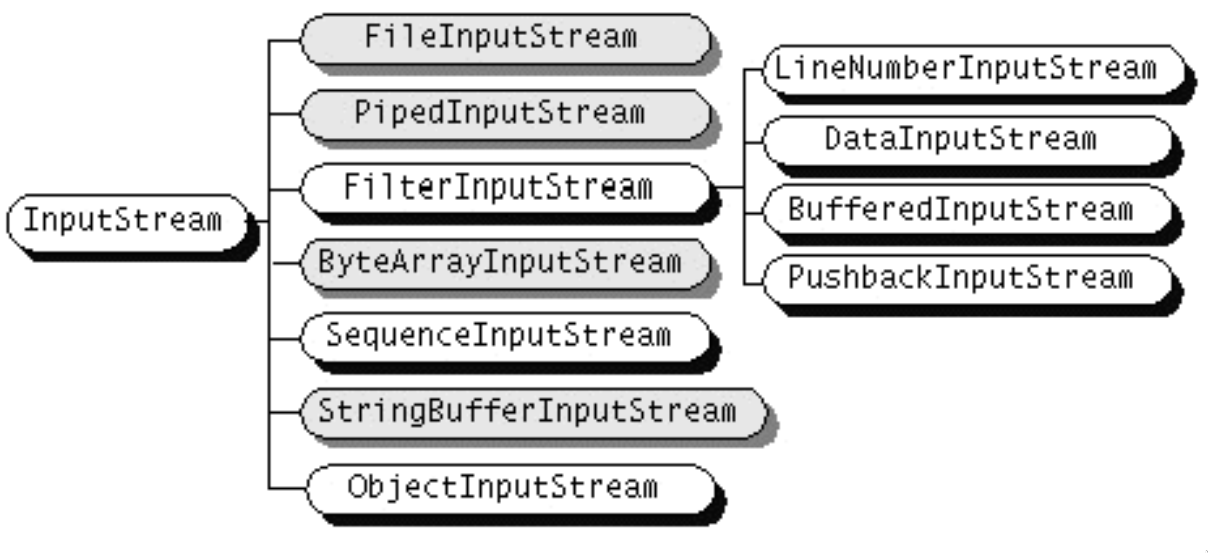
\includegraphics[width=0.7\textwidth]{./images/InputStream.png}
    \caption{Data Sink \& Processing Subclasses of \texttt{InputStream}}
\end{figure}
\begin{figure}[H]
    \centering
    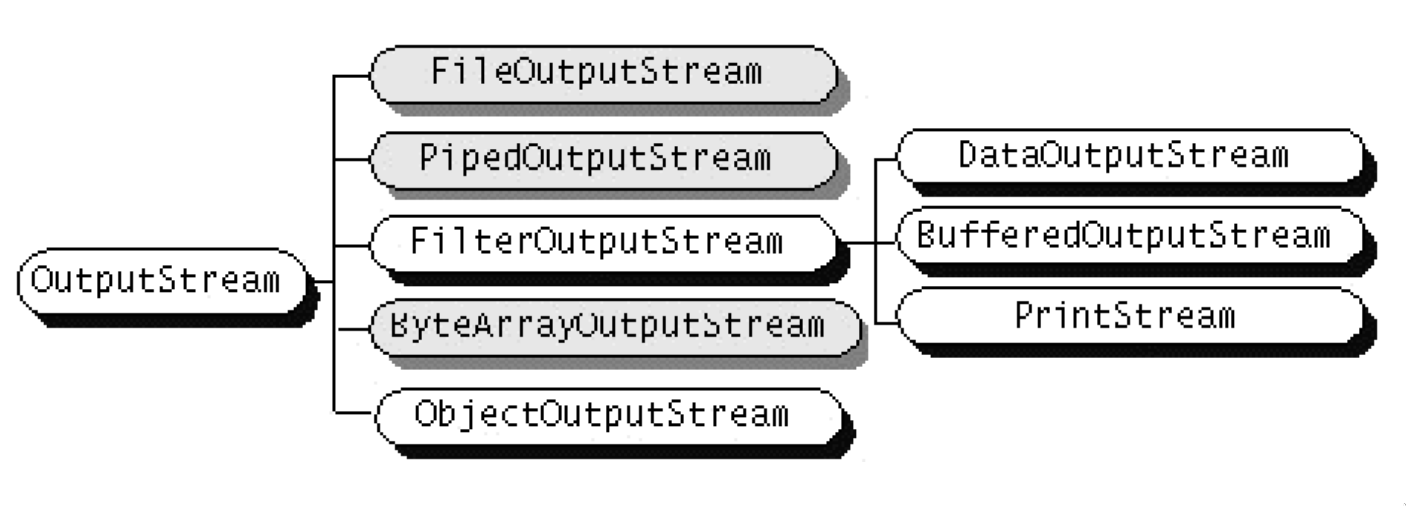
\includegraphics[width=0.7\textwidth]{./images/OutputStream.png}
    \caption{Data Sink \& Processing Subclasses of \texttt{OutputStream}}
\end{figure}

\subsection{Character Streams}
\verb|Reader| \& \verb|Writer| are the abstract superclasses for character streams in \verb|java.io.*|. 
\verb|Reader| provides the API \& partial implementation for readers, i.e. streams that read 16-bit Unicode 
characters and \verb|Writer| provides the API \& partial implementation for writers, i.e. streams that write 
16-bit characters. 
Subclasses of \verb|Reader| \& \verb|Writer| implement specialised streams.
\\\\ 
The following figures show the readers or writers that read/write to/from data sinks in grey, and those that 
performs some sort of processing are shown in white:
\begin{figure}[H]
    \centering
    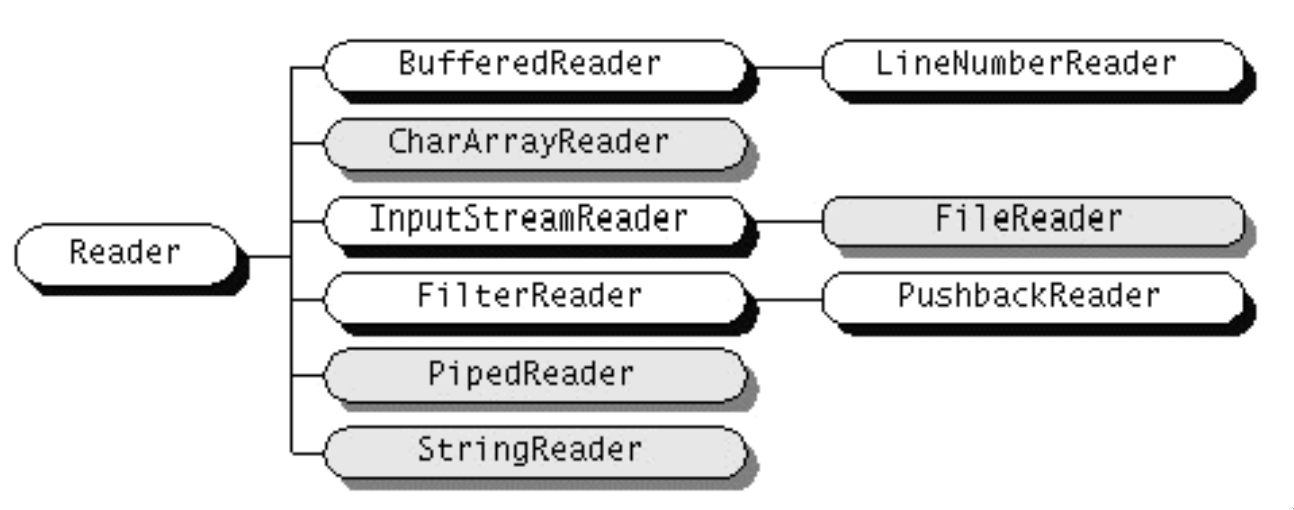
\includegraphics[width=0.7\textwidth]{./images/Reader.png}
    \caption{Data Sink \& Processing Subclasses of \texttt{Reader}}
\end{figure}
\begin{figure}[H]
    \centering
    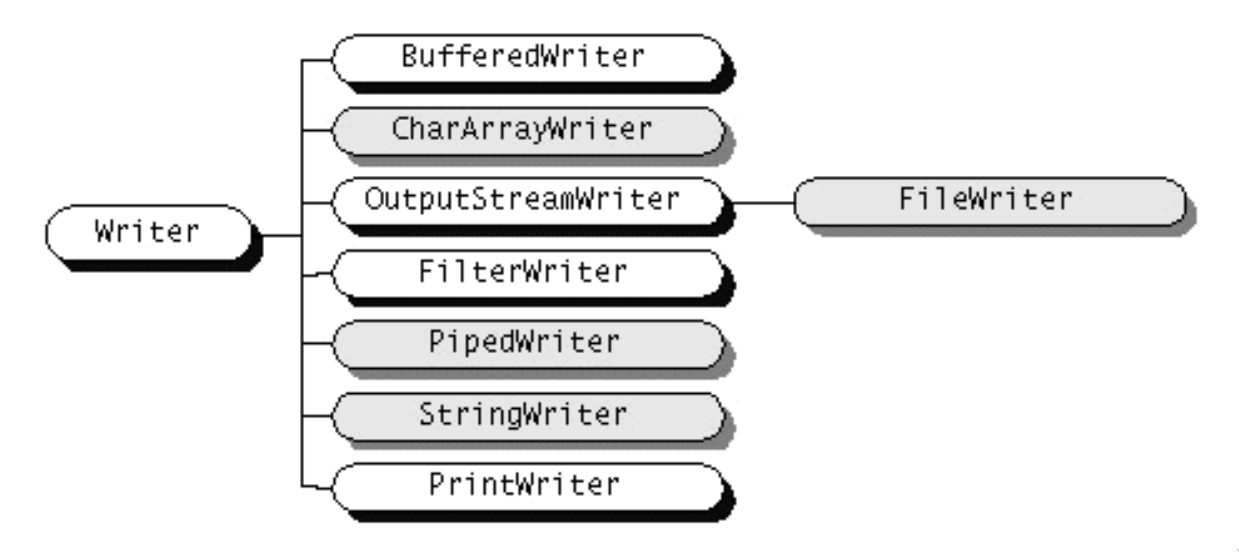
\includegraphics[width=0.7\textwidth]{./images/Writer.png}
    \caption{Data Sink \& Processing Subclasses of \texttt{Writer}}
\end{figure}

Most programs should use readers \& writers to read \& write information because they can handle any character 
in the Unicode character set whereas byte streams are limited to ISO-Latin-1 8-bit bytes.

\subsection{\texttt{Scanner}}
The \textbf{\texttt{Scanner}} class is in the \verb|java.util| package but can be passed an \verb|InputStream| as a 
constructor parameter.
Scanners are often used for reading from the console, i.e. the \verb|System.in| InputStream.
They are used for working with inputs of formatted data consisting of primitive types \& Strings. 
Scanners translate the input to tokens based on their data type and using a delimiter pattern.
They also have a collection of \verb|next()| methods for different data types.

\subsection{Formatting}
\verb|PrintWriter| is a processing character stream that includes common methods for formatting such as 
\verb|print|, \verb|println|, \& \verb|format|.
The \verb|format| method formats multiple arguments based on a \textbf{format String} that includes format specifiers, 
which can be used similar to tokens in Scanners.
See the \verb|java.util.Formatter| class for documentation on format String syntax.

\section{Object Serialization}
The streams \verb|java.io.ObjectInputStream| \& \verb|java.io.ObjectOutputStream| are special in that they can 
read and write actual objects.
The key to writing an object is to represent its state in a serialized form sufficient to reconstruct the object 
as it is read.
Thus reading \& writing objects is a process called \textbf{object serialization}.
Object serialization can be useful in a lot of application domains.
\\\\
Uses of serialization include:
\begin{itemize}
    \item   \textbf{Remote Method Invocation (RMI)}: communication between objects via sockets, e.g. to pass 
            various objects back \& forth between the client \& server.
    \item   \textbf{Lightweight persistence}: the archival of an object for use in a later invocation of the same
            program
\end{itemize}

Reconstructing an object from a stream requires that the object first be written to a stream; writing objects to 
a stream is a straightforward process. 
The following code sample gets the current time in milliseconds by constructing a \verb|Date| object and then
serializes the object.
\begin{code}
\begin{minted}[texcl, mathescape, linenos, breaklines, frame=single]{java}
FileOutputStream out = new FileOutputStream("theTime");
ObjectOutputStream s = new ObjectOutputStream(out);
s.writeObject("Today");
s.writeObject(new Date());
s.flush();
\end{minted}
\caption{Object Serialization Example}
\end{code}

The above code constructs an \verb|ObjectOutputStream| on a \verb|FileOutputStream|, thereby serializing the
object to a file named \verb|theTime|.
Next, the String \verb|Today| \& a \verb|Date| object are written to the stream with the \verb|writeObject|
method of \verb|ObjectOutputStream|.

\subsection{Object Serialization with Related Objects}
if an object refers to other objects, then all of the objects that are reachable from the first must be written
at the same time so as to maintain the relationships between them.
Thus, the \verb|writeObject| method serializes the specified object, traverses its references to other objects 
recursively, and writes them all. 
The \verb|writeObject| method throws a \verb|NotSerializableException| if it's given an object that is not 
serializable.
An object is serializable only if its class implements the \verb|Serializable| interface.

\subsection{Reconstructing Serialized Objects}
Once you've written objects \& primitive data types to a stream, you'll likely want to read them out again and 
reconstruct the objects.
The below code reads in the \verb|String| \& the \verb|Date| object that was written to the file named
\verb|theTime| in the previous example:
\begin{code}
\begin{minted}[texcl, mathescape, linenos, breaklines, frame=single]{java}
FileInputStream in = new FileInputStream("theTime");
ObjectInputStream s = new ObjectInputStream(in);
String today = (String) s.readObject();
Date date = (Date) s.readObject();
\end{minted}
\caption{Object Reconstruction Example}
\end{code}

Note that there is no standard file extension for files that store serialized objects.
\\\\
Like \verb|ObjectOutputStream|, \verb|ObjectInputStream| must be constructed on another stream. 
In this example, the objects were archived in a file, so the code constructs an \verb|ObjectInputStream| on a 
\verb|FileInputStream|.
Next, the code uses the \verb|readObject| of the \verb|ObjectInputStream| method to read the \verb|String| \& 
\verb|Date| objects from the file.
The objects must be read from the stream in the same order in which they were written.
Note that the return value from \verb|readObject| is an object that is cast to and assigned to a specific type.
The \verb|readObject| method deserializes the next object in the stream and traverses its references to other 
objects recursively to deserialize all objects that are reachable from it.
In this way, it maintains the relationships between objects.
The methods in \verb|DataInput| parallel those defined in \verb|DataOutput| for writing primitive data types.

\subsection{Serializing Classes}
AN object is serializable only its class implements the \verb|Serializable| interface. 
Thus, if you want to serialize an instance of one of your classes, the class must implement the 
\verb|Serializable| interface, i.e. it must have the \mintinline{java}{implements Serializable} clause. 
\verb|Serializable| is an empty interface, i.e. it does not contain any method declarations; its purpose is 
simply to identify classes whose objects are serializable.
Its complete definition is as follows:
\begin{code}
\begin{minted}[texcl, mathescape, linenos, breaklines, frame=single]{java}
package java.io;

public interface Serializable {
    // there's nothing in here!
};
\end{minted}
\caption{Definition of the \texttt{Serializable} Interface}
\end{code}

You don't have to write any methods to make a class serializable.
The serialization of instances of a serializable class are (by default) handled by the \verb|defaultWriteObject| 
method of the \verb|ObjectOutputStream|.
\\\\
All instance variables of a class must be serialized for it to be serializable, including referenced objects 
\& those within referenced data structures
In Java, all primitive type variables are serializable by default.
We can ignore instance variables in the process by declaring them as \verb|transient|

\subsection{The \texttt{defaultWriteObject} Method}
The \verb|defaultWriteObject| method automatically writes out everything required to reconstruct an instance
of the class, including the class of the object, the class signature, and values of non-transient \& non-static
members, including members that refer to other objects.
For many classes, the default behaviour is fine. 
However, default serialization can be slow, and a class might want more explicit control over the serialization.

\subsection{Customising Serialization}
You can customise serialization for your classes by providing two methods: \verb|writeObject| \&
\verb|readObject|.
The \verb|writeObject| method controls what information is saved and is typically used to append additional 
information to the stream.
The \verb|readObject| method either reads the information written by the corresponding \verb|writeObject|
method or can be used to update the state of the object after it has been restored.
\\\\
The \verb|writeObject| method must be declared exactly as follows.
Note that it should call the stream's \verb|defaultWriteObject| as the first thing it does to perform
default serialization (any special arrangements can be handled afterwards):
\begin{code}
\begin{minted}[texcl, mathescape, linenos, breaklines, frame=single]{java}
ptivate void writeObject(ObjectOutputStream s) throws IOException {
    s.defaultWriteObject();
    // customised serialization code
}
\end{minted}
\caption{Declaration of the \texttt{writeObject} Method}
\end{code}

The \verb|readObject| method must read in everything written by \verb|writeObject| in the same order in which
it was written.
The following \verb|readObject| method corresponds to the above \verb|writeObject| method:
\begin{code}
\begin{minted}[texcl, mathescape, linenos, breaklines, frame=single]{java}
private void readObject(ObjectInputStream s) throws IOException {
    s.defaultReadObject();
    // customised deserialization code
    // followed by code to update the object if necessary
}
\end{minted}
\caption{Declaration of the \texttt{readObject} Method}
\end{code}

The \verb|readObject| method can also perform calculations or update the state of the object in some way.
The \verb|writeObject| \& \verb|readObject| methods are responsible for serializing only the immediate class.
Any serialization required for the superclasses is handled automatically.
However, a class that needs to explicitly co-ordinate with its superclasses to serialize itself can do so by 
implementing the \verb|Externalizable| interface.

\subsubsection{The \texttt{Externalizable} Interface}
For complete, explicit control over the serialization process, a class must implement the
\verb|Externalizable| interface.
For \verb|Externalizable| objects, only the identify of the object's class is automatically saved by the 
stream.
The class is responsible for reading \& writing its contents, and it must co-ordinate with its superclasses
to do so

\section{Random File Access}
The input \& output streams that we have been dealing with so far have been \textbf{sequential access streams}, 
i.e. streams whose contents must be read or written sequentially.
Sequential access files are a hangover from sequential media such as magnetic tape, but are still very useful
today.
\textbf{Random access files} permit non-sequential (or random) access to the contents of a file.

\subsection{Random File Access Example Use Case}
Consider the ``zip'' archive format.
Zip archives contain files and are typically compressed to save space.
Zip archives also contain a \verb|dir-entry| at the end of the file that indicates where the various files
contained within the zip archive begin:
\begin{figure}[H]
    \centering
    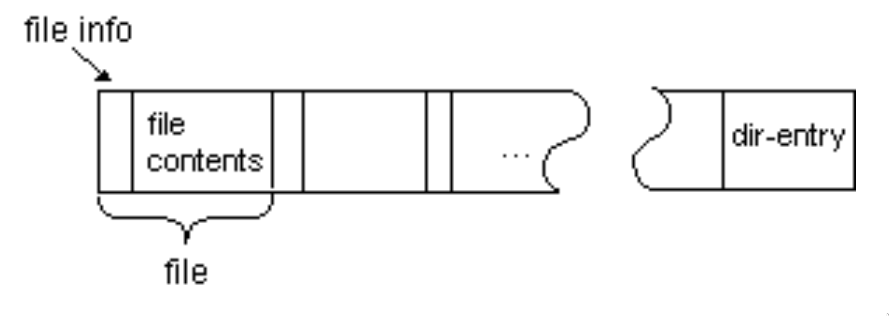
\includegraphics[width=0.7\textwidth]{./images/dir-entry.png}
    \caption{Zip Archive Format}
\end{figure}

Suppose that you want to extract a specific file from a zip archive.
If you use a sequential access stream, you have to do the following:
\begin{enumerate}
    \item   Open the zip archive.
    \item   Search through the zip archive until you have located the file that you want to extract.
    \item   Extract the file.
    \item   Close the zip archive.
\end{enumerate}

Using this algorithm, you'd have to read half the zip archive on average before finding the file that you 
want to extract.
You can extract the same file from the zip archive more efficiently using the \textbf{seek} feature of a 
random access file:
\begin{enumerate}
    \item   Open the zip archive.
    \item   Seek to the \verb|dir-entry| and locate the entry for the file you want to extract from the zip 
            archive.
    \item   Seek backwards within the zip archive to the position of the file to extract.
    \item   Extract the file 
    \item   Close the zip archive.
\end{enumerate}

This algorithm is more efficient because you only read the \verb|dir-entry| and the file that you want to 
extract.

\subsection{The \texttt{RandomAccessFile} Class}
The \verb|RandomAccessFile| class in the \verb|java.io| package implements a random access file.
Unlike the input \& output stream classes in \verb|java.io|, \verb|RandomAccessFile| is used for both 
reading \& writing files; it implements both the \verb|DataInput| \& \verb|DataOutput| interfaces and therefore
can be used for both reading \& writing.
\\\\
We create \verb|RandomAccessFile| objects with different arguments depending on whether you intend to read or 
write.
\verb|RandomAccessFile| is similar to \verb|FileInputStream| \& \verb|FileOutputStream| in that you specify 
a file on the native file system to open, either with a filename or a \verb|File| object.
When you create \verb|RandomAccessFile|, you must indicate whether you will be reading the file or also
writing to it.
The following code snippet creates a \verb|RandomAccessFile| to read the file named \verb|farrago.txt|:
\begin{minted}[texcl, mathescape, linenos, breaklines, frame=single]{java}
new RandomAccessFile("farrago.txt", "r");
\end{minted}

The following code snippet opens the same file for both reading \& writing:
\begin{minted}[texcl, mathescape, linenos, breaklines, frame=single]{java}
new RandomAccessFile("farrago.txt", "rw");
\end{minted}

After the file has been opened, you can use the common read \& write method to perform I/O on the file. 
The \verb|RandomAccessFile| class supports the notion of a file pointer, which indicates the current location 
in the file.
When the file is first created, the file pointer is \verb|0|, indicating the start of the file.
Calls to the read \& write methods adjust the file pointer by the number of bytes read or written.
\\\\
In addition to the normal file I/O methods that implicitly move the file pointer when the operation occurs, 
\verb|RandomAccessFile| also contains three methods for explicitly manipulating the file pointer:
\begin{itemize}
    \item   \verb|skipBytes()|: moves the file pointer forward the specified number of bytes.
    \item   \verb|seek()|: positions the file pointer just before the specified byte.
    \item   \verb|getFilePointer()|: returns the current byte location of the file pointer.
\end{itemize}

\verb|RandomAccessFile| is somewhat disconnected from the input \& output streams in \verb|java.io|: it 
doesn't inherit from either \verb|InputStream| or \verb|OutputStream|.
This has some disadvantages in that you can't apply the same filters to \verb|RandomAccessFile|s that you can 
However, \verb|RandomAccessFile| does implement the \verb|DataInput| \& \verb|DataOutput| interfaces:
if you design a filter that works for either \verb|DataInput| or \verb|DataOutput|, it will work on any 
\verb|RandomAccessFile|.

\section{Type-Wrapper Classes}
Collections manipulate \& store \textbf{Objects}, not primitive types.
Each Java primitive type has a corresponding \textbf{type-wrapper class} in \verb|java.lang| that enables primitives to be manipulated as Objects, e.g.
\verb|Boolean|, \verb|Byte|, \verb|Character|, \verb|Double|, \verb|Float|, \verb|Integer|, \verb|Long|, \verb|Short|.
Numeric type-wrapper classes extend the \verb|Number| class.
Methods related to primitive types are contained in the type-wrapper classes, e.g. \verb|parseInt| is located in the class \verb|Integer|.

\subsection{Autoboxing \& Auto-Unboxing}
A \textbf{boxing conversion} converts a value of a primitive type to an Object of the corresponding type-wrapper class.
An \textbf{unboxing conversion} converts an object of a type-wrapper class to a value of the corresponding primitive type.
When these conversions are done automatically, they are referred to as \textbf{autoboxing} \& \textbf{auto-unboxing}.
For example:
\begin{minted}[texcl, mathescape, linenos, breaklines, frame=single]{java}
Double[] myDoubles = new Double[10];
myDoubles[0] = 22.7;                    // autoboxed to a Double Object
double firstDoubleValue = myDoubles[0]; // auto-unboxed to a double primitive
\end{minted}

\section{Collections}
A \textbf{Collection} (sometimes called a container) is an object that groups multiple elements into a single unit.
Collections are used to store, retrieve, \& manipulate data, and to transmit data from one method to another. 
Collections typically represent data items that form a natural group.

\subsection{Interfaces}
The core Collections interfaces are the interfaces used to manipulate Collections, and to pass them from one method to another. 
The basic purpose of these interfaces is to allow Collections to be manipulated independently of the details of their representations.
The core Collections interfaces are the main foundation of the Collections framework.

\begin{figure}[H]
    \centering
    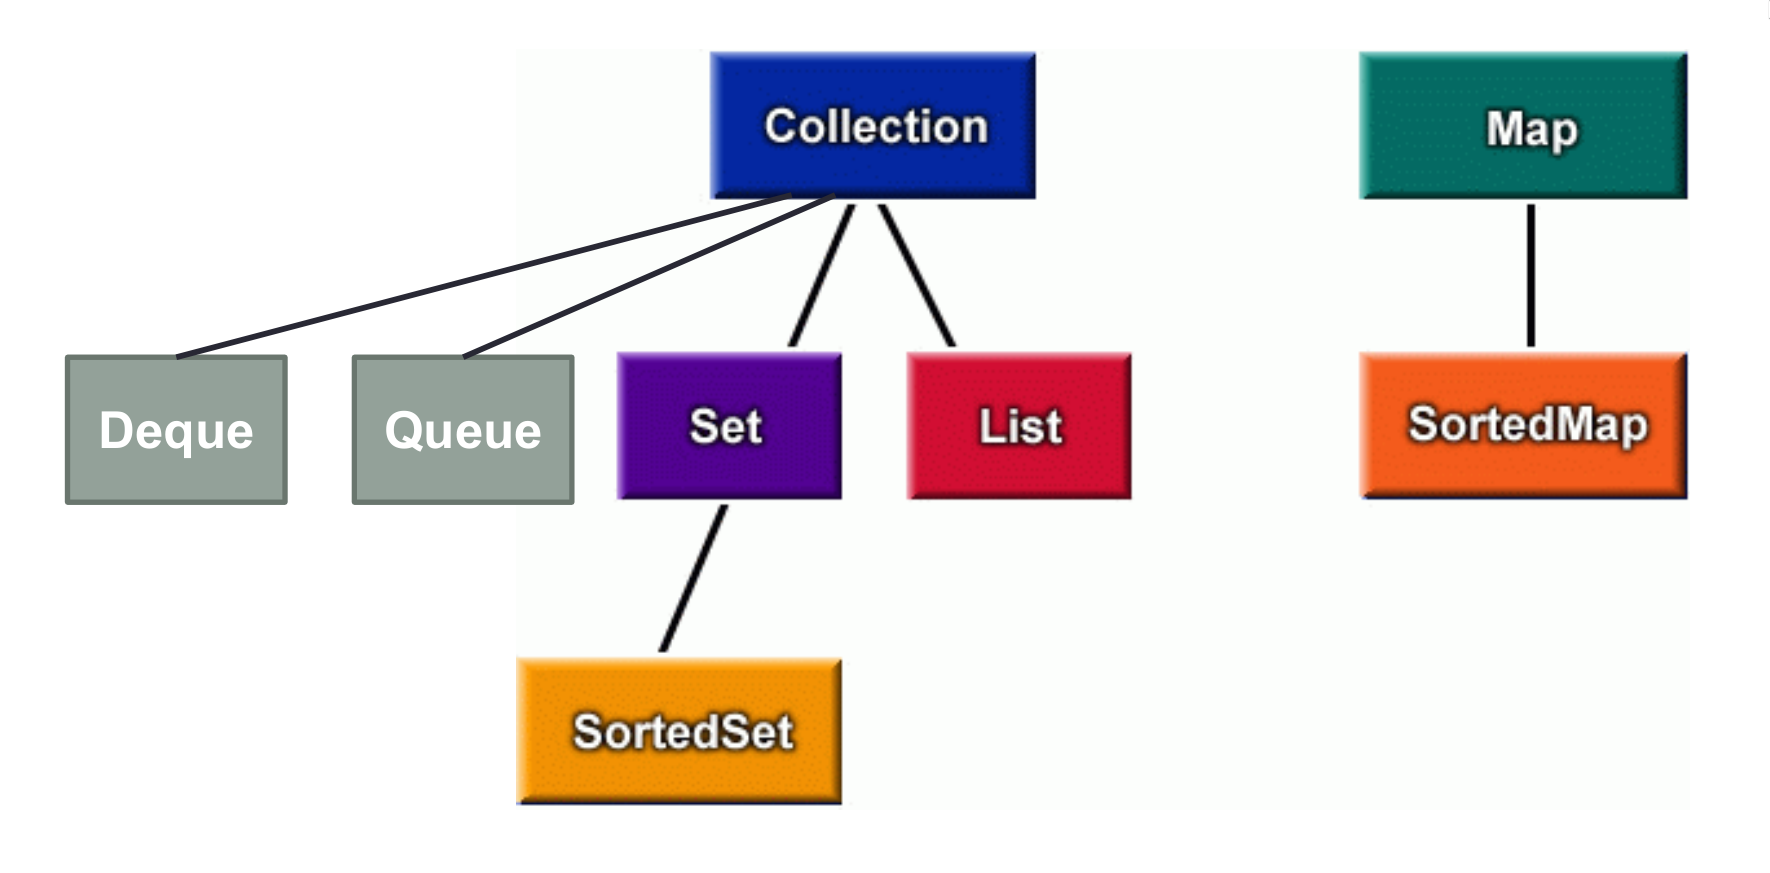
\includegraphics[width=0.7\textwidth]{./images/core_collections_interfaces.png}
    \caption{Core Collections Interfaces}
\end{figure}

The core collection interfaces form a hierarchy: a \verb|Set| is a special kind of \verb|Collection|, a \verb|SortedSet| is a special kind of \verb|Set|, etc.
Note that the hierarchy consists of two distinct trees: a \verb|Map| is not a true \verb|Collection|.
\\\\
To keep the number of core collection interfaces manageable, the JDK doesn't provide separate interfaces for each variant of each collection type.
Among the possible variants are immutable, fixed-size, \& append-only.
Instead, the modification operations in each interface are designated optional, i.e. a given implementation does not have to support all of these operations.
If an unsupported operation is invoked, the Collection will throw an \verb|UnsupportedOperationException|.
Implementations are responsible for documenting which of the optional operations they support. 
All of the JDK's general-purpose implementations support all of the optional operations.

\subsubsection{The \texttt{Collection} Interface}
The \verb|Collection| interface is the root of the Collection hierarchy.
A \verb|Collection| represents a group of objects, which are known as \emph{elements}.
Some \verb|Collection| implementations allow duplicate elements, while others do not; some \verb|Collection| implementations are ordered, and others are not.
The JDK doesn't provide any direct implementations of this interface: it provides only implementations of the more specific sub-interfaces like \verb|Set| \& 
\verb|List|.
\\\\
The \verb|Collection| interface is the lowest common denominator that all Collections implement.
It is used to pass Collections around and to manipulate them when maximum generality is desired.

\begin{code}
\begin{minted}[texcl, mathescape, linenos, breaklines, frame=single]{java}
public interface Collection {
    // Basic Operations
    int size();
    boolean isEmpty();
    boolean contains(Object element);
    boolean add(Object element);        // Optional
    boolean remove(Object element);     // Optional
    Iterator iterator();

    // Bulk Operations
    boolean containsAll(Collection c);
    boolean addAll(Collection c);       // Optional
    boolean removeAll(Collection c);    // Optional
    boolean retainAll(Collection c);    // Optional
    void clear();                       // Optional        

    // Array Operations
    Object[] toArray();
    Object[] toArray(T[] a);
}
\end{minted}
\caption{The \texttt{Collection} Interface}
\end{code}

\section{Graphical User Interfaces}
\textbf{Graphical User Interfaces (GUIs)} give a program a distinctive ``look \& feel'', provide users with 
a basic level of familiarity, and are built from GUI components such as controls, widgets, etc.
The user interacts with GUI components via the mouse, keyboard, etc.

\subsection{Swing}
\textbf{Swing} GUI components are from the package \verb|javax.swing|. 
They are lightweight components written entirely in Java.
The components originate from AWT (\verb|java.awt|).
A common superclass structure of many of the Swing components is: \verb|java.lang.Object| {\rightarrow} 
\verb|java.awt.Component| {\rightarrow} \verb|java.awt.Container| {\rightarrow} \verb|javax.swing.JComponent|.
\\\\
Some basic GUI components include:
\begin{itemize}
    \item   \verb|JLabel|: an area where uneditable text or icons can be displayed.
    \item   \verb|JTextField|: an area in which the user inputs data form the keyboard. Can also display information.
    \item   \verb|JButton|: an area that triggers an event when clicked.
    \item   \verb|JCheckBox|: a GUI component that is either selected or not.
    \item   \verb|JComboBox|: a drop-down list of items from which the user can make a selection by clicking an 
            item in the list or by typing into the box.
    \item   \verb|JPanel|: a container in which components can be placed.
\end{itemize}

\section{INSERT MISSING GUI SHIT HERE}


\section{Multithreaded Programming}
A \textbf{process} is an instance of a program being executed.
A \textbf{multitasking} environment allows multiple process to be ran concurrently. 
(In reality, only one process is running at a given time on a single CPU.
Time slicing between processes makes it appear as if they are all running at the same time.)
\\\\
A \textbf{thread} is a ``lightweight process'', i.e. it does not have all the overhead that a process has.
Both processes \& threads have their own independent CPU state, i.e. they have their own processor stack,
their own instruction pointer, \& their own CPU register values.
Multiple threads can share the same memory address space, i.e. share the same variables.
Processes, on the other hand, generally do not share their address space with other processes.
As a rule of thumb, if an application or applet performs a time-consuming task, it should create and use its own thread of execution 
to perform that task.

\subsection{Threads \& Java}
Java has language-level support for threads and it is therefore easy to create multiple independent threads 
of execution in Java.
Any class that is a subclass of \mintinline{java}{java.lang.Thread} or that implements the 
\mintinline{java}{java.lang.Runnable} interface can be used to create threads.
\\\\
When a program creates a thread, it can pass the \mintinline{java}{Thread} class constructor as an object whose 
statements will be executed.
The program can start a thread's execution by using its \mintinline{java}{start()} method; the 
\mintinline{java}{start()} method will in turn call the \mintinline{java}{Thread} object's
\mintinline{java}{run()} method.


\subsubsection{\texttt{java.lang.Runnable}}
To create a thread, we instantiate the \mintinline{java}{java.lang.Thread} class. 
One of \mintinline{java}{Thread}'s constructors takes objects that implement the \mintinline{java}{Runnable}
interface. 
The \mintinline{java}{Runnable} interface contains only a single method:
\begin{code}
\begin{minted}[texcl, mathescape, linenos, breaklines, frame=single]{java}
public interface Runnable {
    public void run();
}
\end{minted}
\caption{The \texttt{Runnable} interface}
\end{code}


To create a thread, we create an instance of the \mintinline{java}{Thread} class. 
We start the thread by calling the \mintinline{java}{start()} method of the thread, which in turn invokes 
the thread's \mintinline{java}{run()} method. 
The thread will terminate when the \mintinline{java}{run()} method terminates.
\begin{code}
\begin{minted}[texcl, mathescape, linenos, breaklines, frame=single]{java}
class Fred implements Runnable {
    public void run() {
        // insert code to be ran here
    }

    public static void main(String args[]) {
        Thread t = new Thread(new Fred()) {
            t.start();
        }
    }
}
\end{minted}
\caption{Creating \& Starting a Thread}
\end{code}

\subsection{Thread Priority \& Daemons}
Every thread has a \textbf{priority}: threads with higher priority are executed in preference to threads 
with lower priority.
Threads can also be marked as a \textbf{daemon}: a background thread that is not expected to exit.
New threads initially have their priority set to the priority of the creating thread.
The new thread is a daemon thread if \& only if the creating thread is a daemon thread

\subsection{Threads \& the JVM}
When the Java Virtual Machine starts up, there is usually a single non-daemon (user) thread initially; this
thread calls the \mintinline{java}{main()} method of an application.
The JVM continues to execute threads until either the \mintinline{java}{exit()} method of the class 
\mintinline{java}{Runtime} is called or all non-daemon (user) threads have died.

\subsection{Thread Death}
Threads can be killed by calling their \mintinline{java}{stop()} method but this is not a good idea in general. 
It is preferable to have a thread die naturally by having its \mintinline{java}{run()} return. 
This is often done by altering some variable that causes a while loop to terminate in the \mintinline{java}{run()}
method.

\subsection{Synchronisation}
Multithreaded programming requires special care, and is generally more difficult to debug.
We want to prevent multiple threads from altering the state of an object at the same time.
Sections of code that should not be executed simultaneously are called \textbf{critical sections}.
We want to have \textbf{mutual exclusion} of concurrent threads in critical sections of code.
In Java, this is done by using \textbf{synchronised methods} or \textbf{synchronised statements}.

\subsubsection{The \texttt{synchronized} Statement}
A \mintinline{java}{synchronized} statement attempts to acquire a \textbf{lock} for the object or array 
specified by the \mintinline{java}{expression}.










\end{document}
